\documentclass{standalone}
\usepackage[utf8]{inputenc}
\usepackage{tikz}

\begin{document}
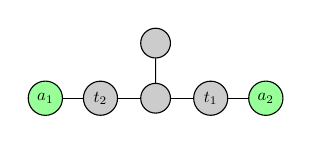
\begin{tikzpicture}[scale=.7,every node/.style = {scale=.6,draw,shape=circle, align=center, fill=gray!30}, level/.style={sibling distance=2.5cm/#1,level distance=1.0cm}]]
	\node[fill=green!40] (v1) at (0,0){$a_1$};
	\node[fill=gray!40] (v2) at (1,0) {$t_2$};
	\node[fill=gray!40] (v3) at (2,0) {~~~};
	\node[fill=gray!40] (v4) at (3,0) {$t_1$};
	\node[fill=green!40] (v5) at (4,0) {$a_2$};
	\node[fill=gray!40] (v6) at (2,1) {~~~};

 \foreach \from\to in {v1/v2,v2/v3,v3/v4,v4/v5,v3/v6}
	\draw (\from) edge  (\to);

 \end{tikzpicture}

  \end{document}
